\documentclass[journal,12pt,twocolumn]{IEEEtran}

\usepackage{setspace}
\usepackage{gensymb}
\usepackage{float}
\singlespacing


\usepackage[cmex10]{amsmath}

\usepackage{amsthm}

\usepackage{mathrsfs}
\usepackage{txfonts}
\usepackage{stfloats}
\usepackage{bm}
\usepackage{cite}
\usepackage{cases}
\usepackage{subfig}

\usepackage{longtable}
\usepackage{multirow}

\usepackage{enumitem}
\usepackage{mathtools}
\usepackage{steinmetz}
\usepackage{tikz}
\usepackage{circuitikz}
\usepackage{verbatim}
\usepackage{tfrupee}
\usepackage[breaklinks=true]{hyperref}
\usepackage{graphicx}
\usepackage{graphics}
\usepackage{tkz-euclide}
\usepackage{float}

\usetikzlibrary{calc,math}
\usepackage{listings}
    \usepackage{color}                                            %%
    \usepackage{array}                                            %%
    \usepackage{longtable}                                        %%
    \usepackage{calc}                                             %%
    \usepackage{multirow}                                         %%
    \usepackage{hhline}                                           %%
    \usepackage{ifthen}                                           %%
    \usepackage{lscape}     
\usepackage{multicol}
\usepackage{chngcntr}

\DeclareMathOperator*{\Res}{Res}

\renewcommand\thesection{\arabic{section}}
\renewcommand\thesubsection{\thesection.\arabic{subsection}}
\renewcommand\thesubsubsection{\thesubsection.\arabic{subsubsection}}

\renewcommand\thesectiondis{\arabic{section}}
\renewcommand\thesubsectiondis{\thesectiondis.\arabic{subsection}}
\renewcommand\thesubsubsectiondis{\thesubsectiondis.\arabic{subsubsection}}


\hyphenation{op-tical net-works semi-conduc-tor}
\def\inputGnumericTable{}                                 %%

\lstset{
%language=C,
frame=single, 
breaklines=true,
columns=fullflexible
}
\begin{document}


\newtheorem{theorem}{Theorem}[section]
\newtheorem{problem}{Problem}
\newtheorem{proposition}{Proposition}[section]
\newtheorem{lemma}{Lemma}[section]
\newtheorem{corollary}[theorem]{Corollary}
\newtheorem{example}{Example}[section]
\newtheorem{definition}[problem]{Definition}

\newcommand{\BEQA}{\begin{eqnarray}}
\newcommand{\EEQA}{\end{eqnarray}}
\newcommand{\define}{\stackrel{\triangle}{=}}
\newcommand\hlight[1]{\tikz[overlay, remember picture,baseline=-\the\dimexpr\fontdimen22\textfont2\relax]\node[rectangle,fill=blue!50,rounded corners,fill opacity = 0.2,draw,thick,text opacity =1] {$#1$};}
\bibliographystyle{IEEEtran}
\providecommand{\mbf}{\mathbf}
\providecommand{\pr}[1]{\ensuremath{\Pr\left(#1\right)}}
\providecommand{\qfunc}[1]{\ensuremath{Q\left(#1\right)}}
\providecommand{\sbrak}[1]{\ensuremath{{}\left[#1\right]}}
\providecommand{\lsbrak}[1]{\ensuremath{{}\left[#1\right.}}
\providecommand{\rsbrak}[1]{\ensuremath{{}\left.#1\right]}}
\providecommand{\brak}[1]{\ensuremath{\left(#1\right)}}
\providecommand{\lbrak}[1]{\ensuremath{\left(#1\right.}}
\providecommand{\rbrak}[1]{\ensuremath{\left.#1\right)}}
\providecommand{\cbrak}[1]{\ensuremath{\left\{#1\right\}}}
\providecommand{\lcbrak}[1]{\ensuremath{\left\{#1\right.}}
\providecommand{\rcbrak}[1]{\ensuremath{\left.#1\right\}}}
\theoremstyle{remark}
\newtheorem{rem}{Remark}
\newcommand{\sgn}{\mathop{\mathrm{sgn}}}
\providecommand{\abs}[1]{\left\vert#1\right\vert}
\providecommand{\res}[1]{\Res\displaylimits_{#1}} 
\providecommand{\norm}[1]{\left\lVert#1\right\rVert}
%\providecommand{\norm}[1]{\lVert#1\rVert}
\providecommand{\mtx}[1]{\mathbf{#1}}
\providecommand{\mean}[1]{E\left[ #1 \right]}
\providecommand{\fourier}{\overset{\mathcal{F}}{ \rightleftharpoons}}
%\providecommand{\hilbert}{\overset{\mathcal{H}}{ \rightleftharpoons}}
\providecommand{\system}{\overset{\mathcal{H}}{ \longleftrightarrow}}
	%\newcommand{\solution}[2]{\textbf{Solution:}{#1}}
\newcommand{\solution}{\noindent \textbf{Solution: }}
\newcommand{\cosec}{\,\text{cosec}\,}
\providecommand{\dec}[2]{\ensuremath{\overset{#1}{\underset{#2}{\gtrless}}}}
\newcommand{\myvec}[1]{\ensuremath{\begin{pmatrix}#1\end{pmatrix}}}
\newcommand{\mydet}[1]{\ensuremath{\begin{vmatrix}#1\end{vmatrix}}}
\numberwithin{equation}{subsection}
\makeatletter
\@addtoreset{figure}{problem}
\makeatother
\let\StandardTheFigure\thefigure
\let\vec\mathbf
\renewcommand{\thefigure}{\theproblem}
\def\putbox#1#2#3{\makebox[0in][l]{\makebox[#1][l]{}\raisebox{\baselineskip}[0in][0in]{\raisebox{#2}[0in][0in]{#3}}}}
     \def\rightbox#1{\makebox[0in][r]{#1}}
     \def\centbox#1{\makebox[0in]{#1}}
     \def\topbox#1{\raisebox{-\baselineskip}[0in][0in]{#1}}
     \def\midbox#1{\raisebox{-0.5\baselineskip}[0in][0in]{#1}}
\vspace{3cm}
\title{ASSIGNMENT 12}
\author{C.RAMYA TULASI}
\maketitle
\newpage
\bigskip
\renewcommand{\thefigure}{\theenumi}
\renewcommand{\thetable}{\theenumi}
Download all python codes from 
\begin{lstlisting}
https://github.com/CRAMYATULASI/ASSIGNMENT12/tree/main/ASSIGNMENT12/CODES
\end{lstlisting}
%
and latex-tikz codes from 
%
\begin{lstlisting}
https://github.com/CRAMYATULASI/ASSIGNMENT12/tree/main/ASSIGNMENT12
\end{lstlisting}
%
\section{Question No. 2.32}
A toy company manufactures two types of dolls, A and B. Market research and available resources have indicated that the combined production level should not exceed 1200 dolls per week and the demand for dolls of type B
is at most half of that for dolls of type A.Further, the production level of dolls of type A can exceed three times the production of dolls of other type by at most 600 units. If the company makes profit of Rs 12 and Rs 16 per doll respectively on dolls A and B, how many of each should be produced weekly in order to maximise the profit?
%
\section{Solution}
Let $x$ and $y$ be number of dolls of type $A$ and $B$ respectively such that 
\begin{align}
    x \geq 0 \\
    y \geq 0 
\end{align}
According to the question,
\begin{align}
    x+y &\leq 1200 
\end{align}
\begin{align}
   x-3y &\leq 600 
\end{align}
\begin{align}
-x+2y&\leq 0
\end{align}
$\therefore$ 
\begin{align}
        \max_{\vec{x}} Z &= \myvec{12 & 16}\vec{x}
\end{align}
$\therefore$ Our problem is
\begin{align}
        \max_{\vec{x}} Z &= \myvec{12 & 16}\vec{x}\\
        s.t. \quad 
        \myvec{1 & 1 \\ 1 & -3 \\ -1 & 2 }\vec{x} &\preceq \myvec{1200\\600\\0}
\end{align}

Lagrangian function is given by
\begin{equation}
\begin{aligned}
    &L(\vec{x},\boldsymbol{\lambda}) \\ &= \myvec{12 & 16}\vec{x}+\lcbrak{\sbrak{\myvec{1 & 1}\vec{x}-1200}} \\ &+ \sbrak{\myvec{1 & -3}\vec{x}-600} +\sbrak{\myvec{-1 & 2}\vec{x}} \\ &+ \sbrak{\myvec{-1 & 0}\vec{x}} +\rcbrak{\sbrak{\myvec{0 & -1}\vec{x}}}\boldsymbol{\lambda}
\end{aligned}
\end{equation}
where,
\begin{align}
    \boldsymbol{\lambda} &= \myvec{\lambda_1 \\ \lambda_2 \\ \lambda_3 \\ \lambda_4 \\ \lambda_5 \\ \lambda_6}
\end{align}

Now,
\begin{align}
    \nabla L(\vec{x},\boldsymbol{\lambda}) &= \myvec{12+ \myvec{1 & 1 & 2 & -1 & 0 }\boldsymbol{\lambda}\\ 16+\myvec{1 & -3 & -1 & 0 & -1}\boldsymbol{\lambda} \\ \myvec{1 & 1}\vec{x}-1200 \\ \myvec{-1 & -3}\vec{x}-600 \\ \myvec{-1 & 2}\vec{x}\\ \myvec{-1 & 0}\vec{x} \\ \myvec{0 & -1}\vec{x}}
\end{align}

$\therefore$ Lagrangian matrix is given by
\begin{align}
    \myvec{0 & 0 & 1 & 1 & 2 & -1 & 0 \\ 0 & 0 & 1 & -3 & -1 & 0 & -1 \\ 1 & 1 & 0 & 0 & 0 & 0 & 0 \\ 1 & -3 & 0 & 0 & 0 & 0 & 0 \\ -1 & 2 & 0 & 0 & 0 & 0 & 0 \\ -1 & 0 & 0 & 0 & 0 & 0 & 0 \\ 0 & -1 & 0 & 0 & 0 & 0 & 0 }\myvec{\vec{x} \\ \boldsymbol{\lambda} } &= \myvec{-12 \\ -16 \\ 1200 \\ 600 \\ 0 \\ 0 \\0 }
\end{align}
Considering $\lambda_1,\lambda_2$ as only active multiplier,
\begin{align}
    \myvec{0 & 0 & 1 & 2 \\ 0 & 0 & 1 & -1 \\ 1 & 1 & 0 & 0 \\ -1 & 2 & 0 & 0}\myvec{\vec{x}\\ \boldsymbol{\lambda}} &= \myvec{-12 \\ -16 \\ 1200 \\ 0}
\end{align}
resulting in,
\begin{align}
    \myvec{\vec{x} \\ \boldsymbol{\lambda}} &= \myvec{0 & 0 & 1 & 2 \\ 0 & 0 & 1 & -1 \\ 1 & 1 & 0 & 0 \\ -1 & 2 & 0 & 0}^{-1}\myvec{-12 \\ -16 \\ 1200 \\ 0}
    \\
    \implies   \myvec{\vec{x} \\ \boldsymbol{\lambda}} &= \myvec{0 & 0 & \frac{2}{3} & \frac{-1}{3} \\ 0 & 0 & \frac{1}{3} & \frac{1}{3} \\ \frac{1}{3} & \frac{2}{3} & 0 & 0 \\ \frac{1}{3} & \frac{-1}{3} & 0 & 0}\myvec{-12 \\ -16 \\ 1200 \\ 0}
    \\
    \implies \myvec{\vec{x} \\ \boldsymbol{\lambda}} &= \myvec{800 \\ 400 \\ \frac{-44}{3} \\ \frac{4}{3} }
\end{align}
$\because \boldsymbol{\lambda}=\myvec{\frac{-44}{3} \\ \frac{4}{3}} \succ \vec{0}$ 
\\
$\therefore$ Optimal solution is given by
\begin{align}
    \vec{x} &= \myvec{800\\400} \\
    Z &= \myvec{12 & 16}\vec{x} \\
    &= \myvec{12 & 16}\myvec{800 \\ 400} \\
    &= 16000
\end{align}
By using cvxpy in python ,
\begin{align}
    \vec{x}=\myvec{800.00001236\\399.99998704}\\
    Z = 15999.99994089
\end{align}
Hence ,the profit will be maximum if company produces.
Type A dolls = \boxed{800},
Type B dolls = \boxed{400}.
\numberwithin{figure}{section}
\begin{figure}[H]
\centering
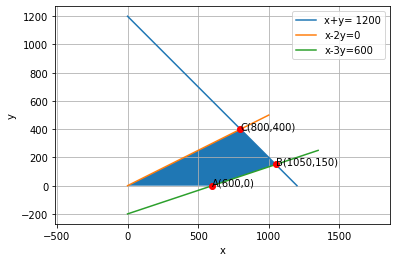
\includegraphics[width=\columnwidth]{download.png}
\caption{TOY PROBLEM}
\label{fig:TOY PROBLEM}	
\end{figure}
\end{document}
